\chapter{Results and discussion}
\label{chap:results}

Our approach on the integration of Embree into ART, as outlined in the previous chapter, was tested on a variety of provided scene files. This chapter provides an overview and analysis of the performance of our implementation. It is decided into three subsections. Subsection \ref{sec:results_csg} discusses the execution time of ART when rendering scenes containing constructive solid geometry. A comparison is drawn between our two approaches for the realization of CSG operations with Embree, the initialization of an entire CSG as a user defined geometry and the traversal through the original scene graph or the dedicated KD tree. We will exclude the provision of results of rendering CSG through the collection of intersection points and their subsequent evaluation, outlined in Subsection \ref{subsec:marteka}. This exclusion is due to the immense increase of rendering time resulting from this approach, which makes this it impractical.

Furthermore, we decided to test our implementation on virtual scenes, not necessarily containing CSG, in order to analyze the overall performance of rendering simple indexed geometries and user defined geometries. Section \ref{sec:result_normal} provides the results on various scenes rendered by an implementation combining Approach 2 and Approach 3, outlined in Subsections \ref{subsec:apprach2} and \ref{subsec:apprach3}. 

Finally, our implementation was tested on scenes, each containing triangle meshes of increasing triangle sizes. The outcome of these experiments is provided and evaluated in Section \ref{sec:result_meshes}. Although this thesis focuses on the implementation of CSG operations, we do not want to withhold these results from the reader because the image synthesis of complex scenes containing large polygon meshes is a crucial use case of Embree.

The following experiments were conducted, if not stated otherwise, on a Asus N551JX laptop, which exhibits a quad-core Intel Core i7–4720HQ processor with a frequency of 2.6 GHz and 8 GB of RAM. The images shown in this chapter were rendered with Embree support at a resolution of 700x700, a path length of 20 and a sample size of 128. The image synthesis of these scenes was performed by using the eight available cores of the machine.

\section{Ray tracing constructive solid geometries}
\label{sec:results_csg}
We tested our implementation of the CSG operations with Embree on six scenes, which were made publicly available by the developers behind ART \footnote{Most of the scenes shown in this chapter can be found in the \texttt{Gallery} folder of the ART repository, which is submitted together with this thesis as an electronic attachment. Scenes or 3D models that are not taken from this folder will be cited.}. All the scenes mentioned in this section contain an infinitie sphere, serving as a sky dome for illuminating the other scene geometry. 
\\

\noindent Here, we provide an overview of the scenes used for testing the CSG operations with Embree:
\begin{itemize}
	\setlength\itemsep{0.05em}
	
	\item The scene shown in Figure \ref{fig:csg_shell} will be referred to as the \textbf{Shell} scene.
	It consists of a single CSG and multiple cube, which are aligned and form the checkerboard pattern, and a procedurally modeled shell. \todo{explain how modeled}
	 This shell is considered a single CSG, therefore only one topmost CSG node associated with it in the scene graph.
	
	
	\item  Figure \ref{fig:csg_orennayar} shows the rendered image of a scene composed of a cylinder, on which three grooved spheres (one example of such a geometry is shown in Figure \ref{fig:art_groovedsphere}) are placed. We call this scene \textbf{Oren-Nayar Spheres} and ON Spheres in Table \ref{tab:csg}, because the purpose of this scene was to showcase ART's implementation of the Oren–Nayar reflectance model \cite{oren1994generalization} with different roughness grades.
	
	\item The \textbf{Villa Rotonda}, shown in the rendered image displayed in Figure \ref{fig:csg_rotonda} is a scene of complex, interleaved CSG. The scene graph for this scene assembled by ART contains only two topmost CSG Nodes whose sub trees represent the entire villa.
	In Table \ref{tab:csg}, we refer to this scene simply as Rotonda.
		
	\item The scene displayed in Figure \ref{fig:csg_torrancesparrow} is composed of twelve grooved spheres that are placed on three deformed cubes with different heights that together form a staircase. Furthermore, a cylinder serves as the ground. We will refer to this scene as \textbf{Torrance-Sparrow Spheres}, and as TS Scene in Table \ref{tab:csg}. The initial purpose of this particular scene was the demonstration of the implementation of the Oren–Nayar reflectance model \cite{torrance1967theory} with varying roughness grades.
	
	\item Figure \ref{fig:csg_plane} shows a rendered image of a scene, composed of a cylinder acting as the ground, and a Biplane, composed of multiple CSG. The total number of topmost CSG nodes in the scene graph, assembled by ART for this particular scene amounts to 28.
	
	\item Lastly, the rendered scene shown in Figure \ref{fig:csg_locomotive} shows a model of an Austrian steam locomotive. The single model is composed of multiple CSG, a total amount of 354 topmost CSG nodes are present in the scene graph associated with this scene.
	
	
\end{itemize}

bla vla vla text bla

\begin{figure}[H]
	\centering
	\subfloat[Shell]{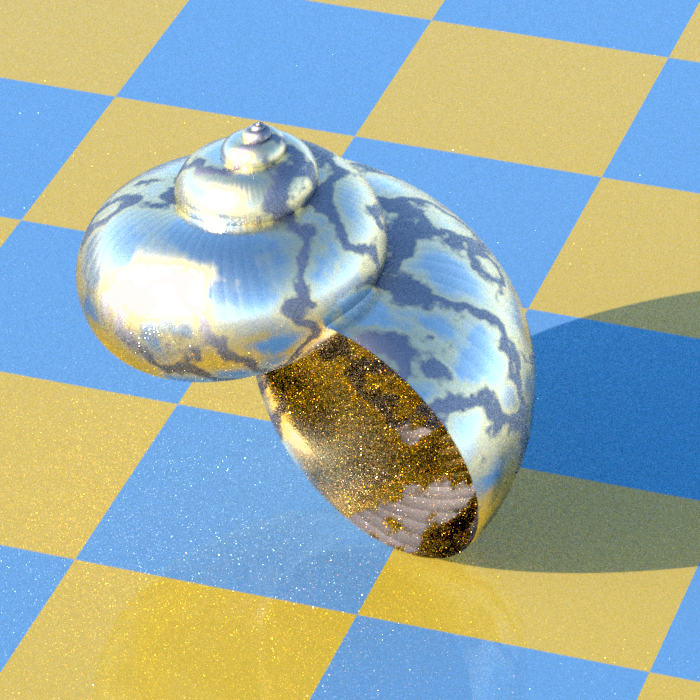
\includegraphics[width=.3\textwidth]{img/4 results/csg/snailEmbree.png}\label{fig:csg_shell}}
	\hfill
	\subfloat[Oren-Nayar Sphreres]{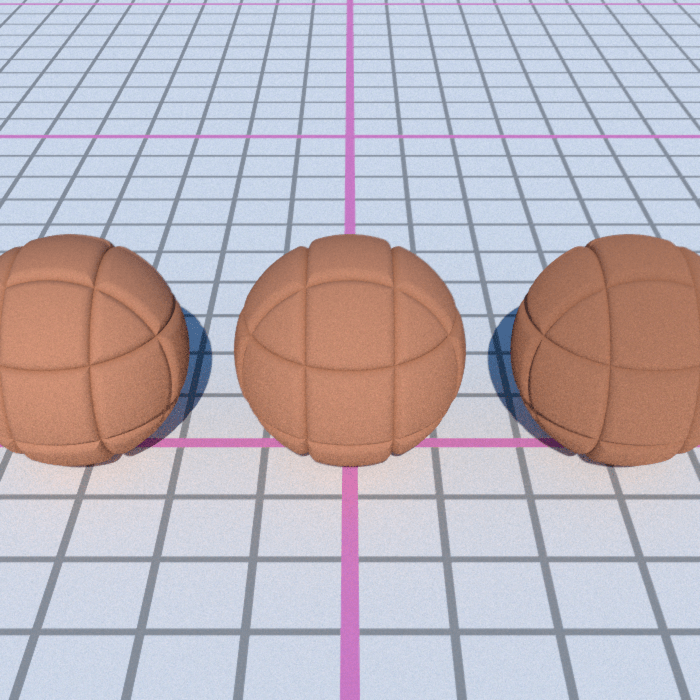
\includegraphics[width=.3\textwidth]{img/4 results/csg/orennayarEmbree.png}\label{fig:csg_orennayar}}
	\hfill
	\subfloat[Villa Rotonda]{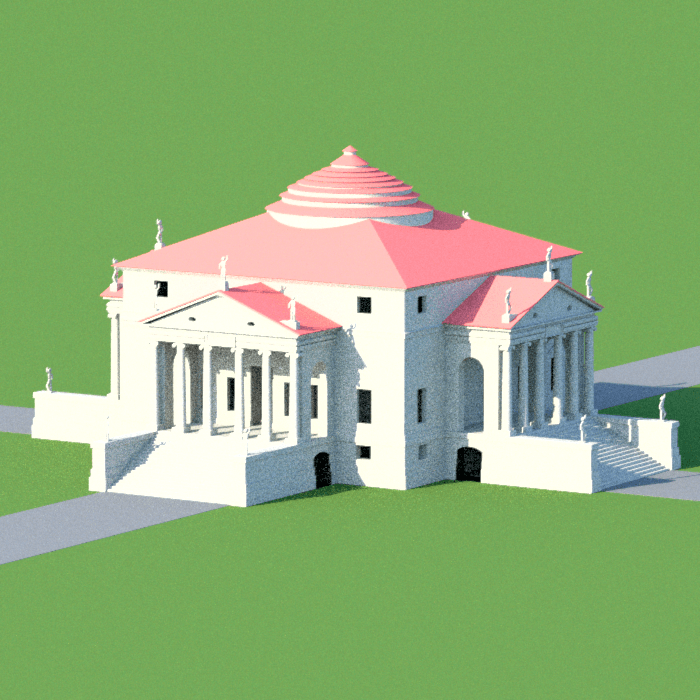
\includegraphics[width=.3\textwidth]{img/4 results/csg/rotondaEmbree.png}\label{fig:csg_rotonda}}
	\\
	\subfloat[Torrance-Sparrow Spheres]{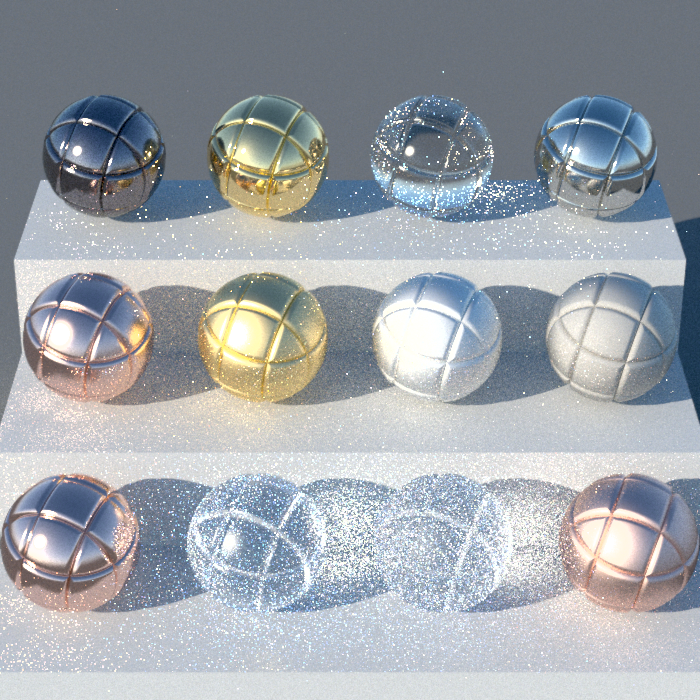
\includegraphics[width=.3\textwidth]{img/4 results/csg/torrancesparrowEmbree.png}\label{fig:csg_torrancesparrow}}
	\hfill
	\subfloat[Parked Biplane]{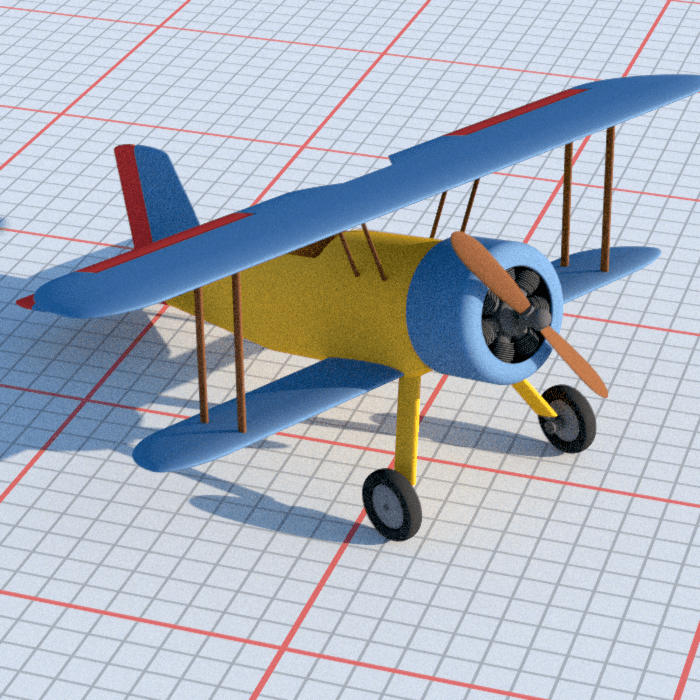
\includegraphics[width=.3\textwidth]{img/4 results/csg/planeEmbree.png}\label{fig:csg_plane}}
	\hfill
	\subfloat[Locomotive]{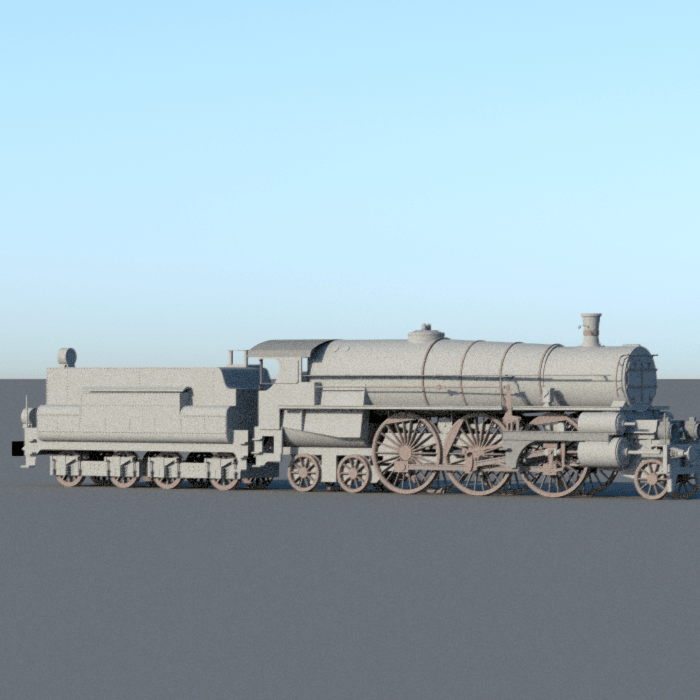
\includegraphics[width=.3\textwidth]{img/4 results/csg/locomotiveEmbree.png}\label{fig:csg_locomotive}}
	
	\caption{Scenes containing CSG, rendered with our implementation.}
	\label{fig:csg_figures}
\end{figure}

\begin{table}[H]
	\centering
	{\footnotesize\sf
		\begin{tabular}{lrrrrrr}
			\toprule
			Scene & \Verb!#!CSG & Native ART & Approach 2 & Speedup 2 & Approach 3 & Speedup 3 \\ 
			\midrule
			Snail & 1 & 2,611.75 sec & 2,437.81 sec & 6.66 \% & 4,151.01 sec & \textcolor{red}{-58.94 \%}  \\
			ON Spheres & 3 & 791.71 sec & 522.97 sec & 33.94 \% & 528.77 sec & 33.21 \% \\
			Rotonda & 2 & 738.25 sec & 629.03 sec & 14.79 \% & 765.44 sec & \textcolor{red}{-3.68 \%}  \\
			\addlinespace % a nice non-intrusive separator of data groups (or final table sums)
			TS Spheres & 12 & 910.56 sec & 896.97 sec & 1.49 \% & 902.61 sec & 0.87 \% \\
			Biplane & 28 & 522.58 sec & 498.25 sec & 4.66 \% & 546.79 sec & \textcolor{red}{-4.63} \% \\
			Locomotive & 354 & 312.94 sec & 272.08 sec & 13.06 \% & 280.83 sec & 10.26 \% \\
			\bottomrule
	\end{tabular}}
	\caption{An example table. Table caption should clearly explain how to interpret the data in the table. Use some visual guide, such as boldface or color coding, to highlight the most important results (e.g., comparison winners).}
	\label{tab:csg}
\end{table}




\section{Final implementation and its performance}
\label{sec:result_normal}

\noindent Here, we provide an overview of the scenes used for testing the overall performance of ART with Embree support:
\begin{itemize}
	\setlength\itemsep{0.05em}
	
	\item
	
	
\end{itemize}


\begin{figure}
	\centering
	\subfloat[Teapot - 4,032 faces]{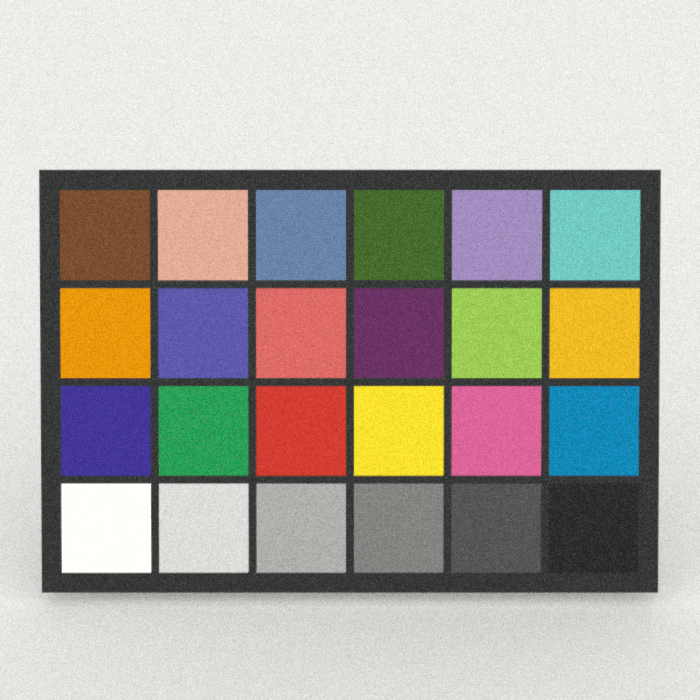
\includegraphics[width=.3\textwidth]{img/4 results/normal/chartEmbree.png}\label{fig:chart}}
	\hfill
	\subfloat[Bunny - 69,451 faces]{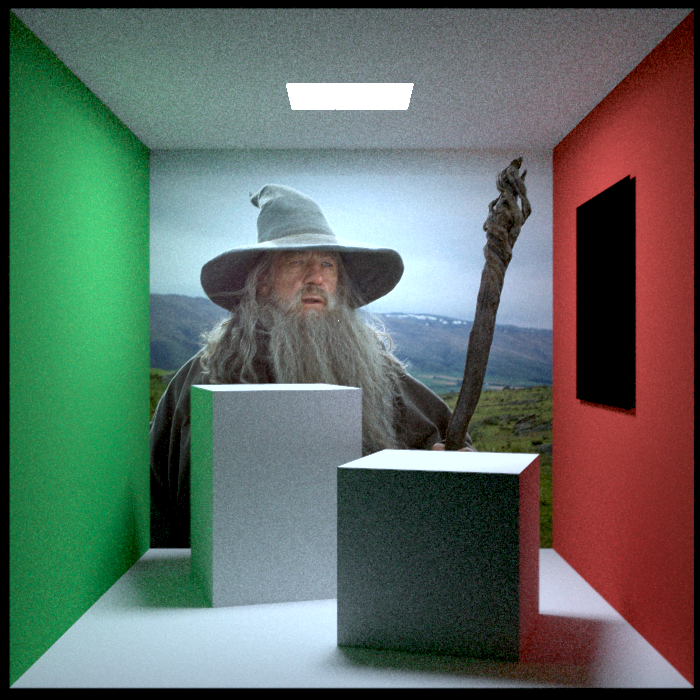
\includegraphics[width=.3\textwidth]{img/4 results/normal/imagemapEmbree.png}\label{fig:gandalf}}
	\hfill
	\subfloat[Michelangelo - 366,011 faces ]{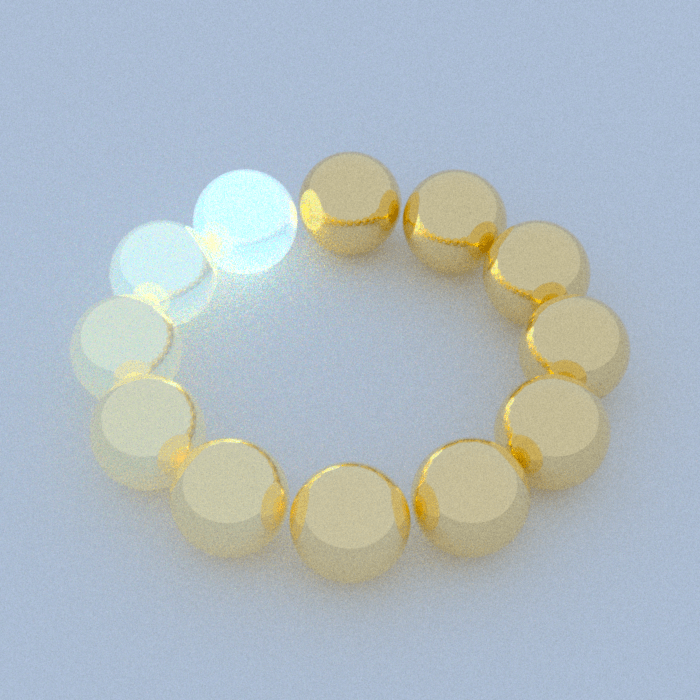
\includegraphics[width=.3\textwidth]{img/4 results/normal/glowEmbree.png}\label{fig:glow}}
	\\
	\subfloat[Happy Buddha - 1,087,716 faces]{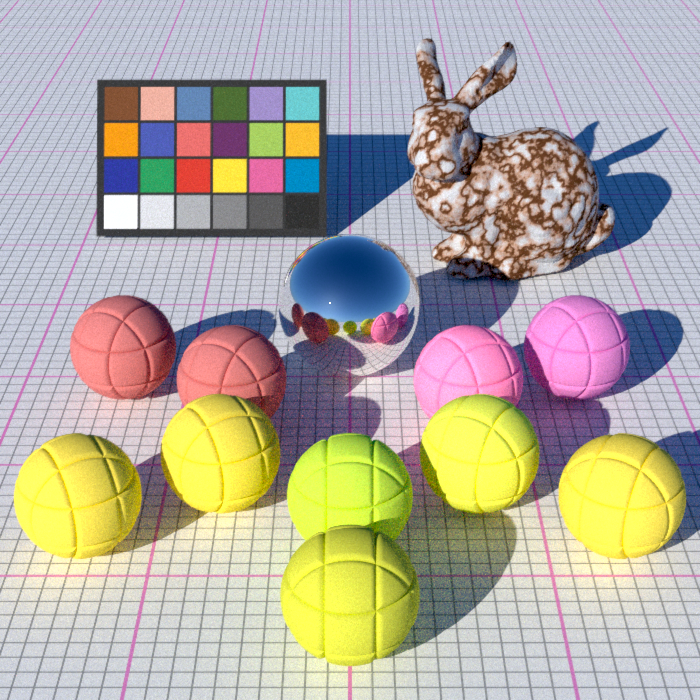
\includegraphics[width=.7\textwidth]{img/4 results/normal/skydomeEmbreeFinal.png}\label{fig:skydome}}

	
	\caption{Scenes from the gallery of the ART repository.}
	\label{fig:scenes}
\end{figure}


\begin{table}
	\centering
	{\footnotesize\sf
		\begin{tabular}{lrrrr}
			\toprule
			Scene & \Verb!#!Geometry & Native ART & Embree & Speedup \\ 
			\midrule
			Figure \ref{fig:chart} & 26 & 196.34 sec & 213.15 sec & \textcolor{red}{-8.56 \%} \\
			Figure \ref{fig:gandalf} & 20 & 485.60 sec & 284.27 sec & 41.46 \% \\
			Figure \ref{fig:glow} & 13 & 401.27 sec & 225.29 sec & 43.86 \%  \\
			Figure \ref{fig:skydome} & 38 & 761.25 sec & 621.96 sec & 18.30 \% \\
			\bottomrule
	\end{tabular}}
	\caption{An example table. Table caption should clearly explain how to interpret the data in the table. Use some visual guide, such as boldface or color coding, to highlight the most important results (e.g., comparison winners).}
	\label{tab:scenes}
\end{table}


\section{Performance of ray tracing triangle meshes}
\label{sec:result_meshes}

\begin{figure}
	\centering
	\subfloat[Teapot - 4,032 faces]{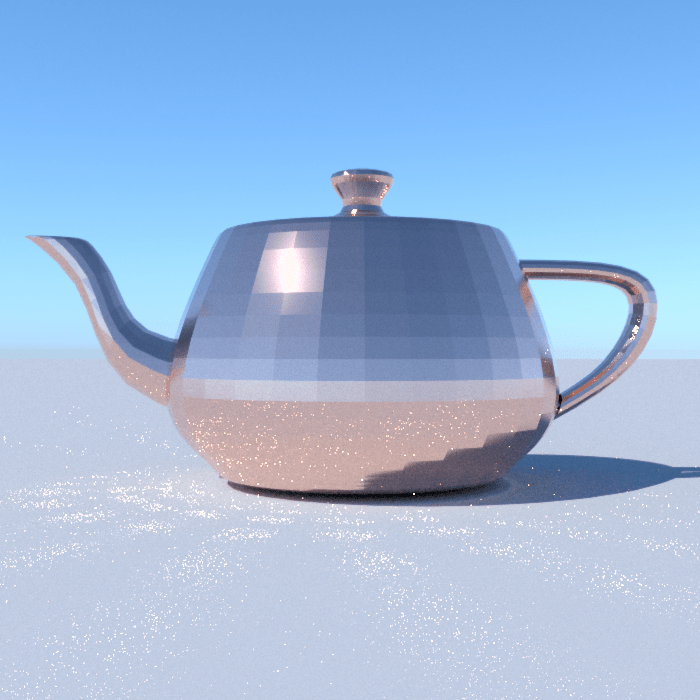
\includegraphics[width=.3\textwidth]{img/4 results/ply/teapotEmbree.png}\label{fig:mesh_teapot}}
	\hfill
	\subfloat[Bunny - 69,451 faces]{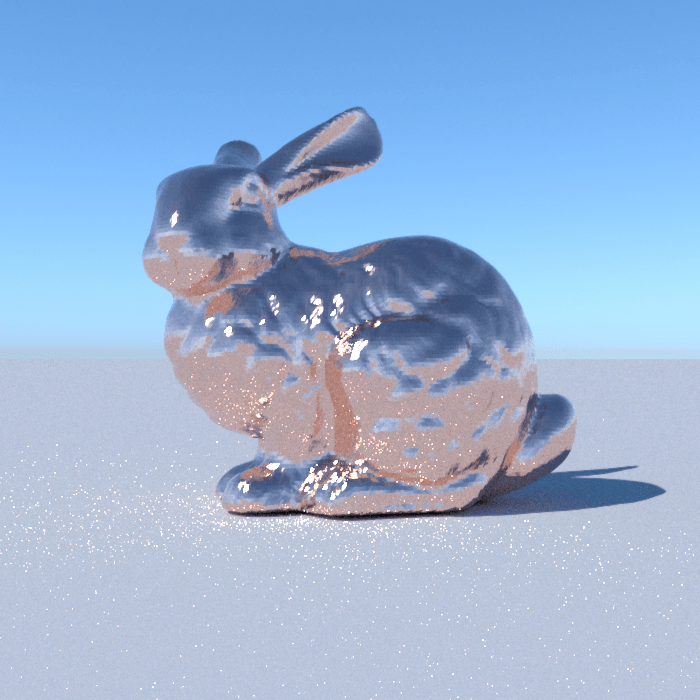
\includegraphics[width=.3\textwidth]{img/4 results/ply/bunnyEmbree.png}\label{fig:mesh_bunny}}
	\hfill
	\subfloat[Michelangelo - 366,011 faces ]{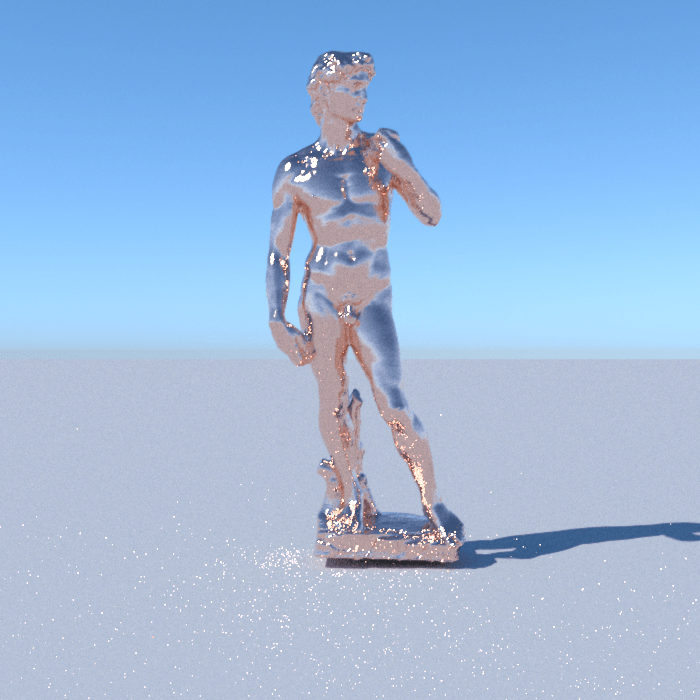
\includegraphics[width=.3\textwidth]{img/4 results/ply/michelangeloEmbree.png}\label{fig:mesh_mike}}
	\\
	\subfloat[Happy Buddha - 1,087,716 faces]{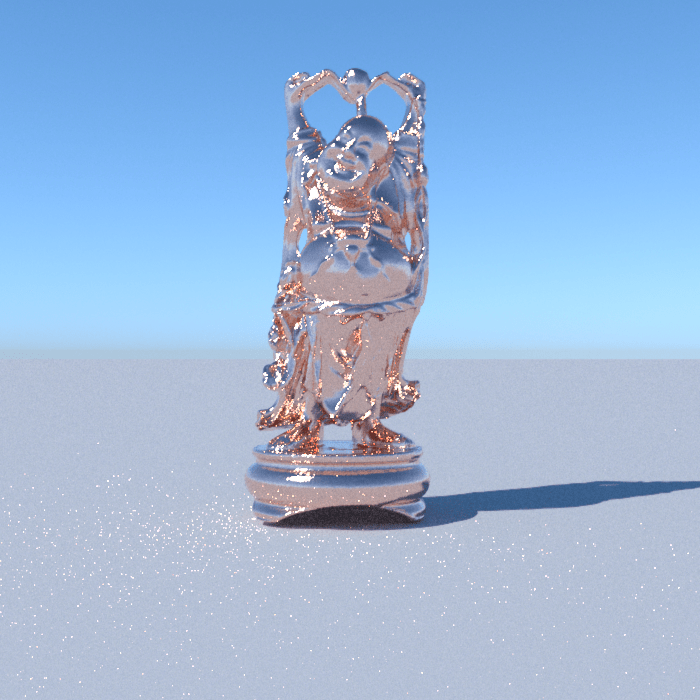
\includegraphics[width=.3\textwidth]{img/4 results/ply/bhuddaEmbree.png}\label{fig:mesh_buddha}}
	\hfill
	\subfloat[Dragon - 7,219,045 faces]{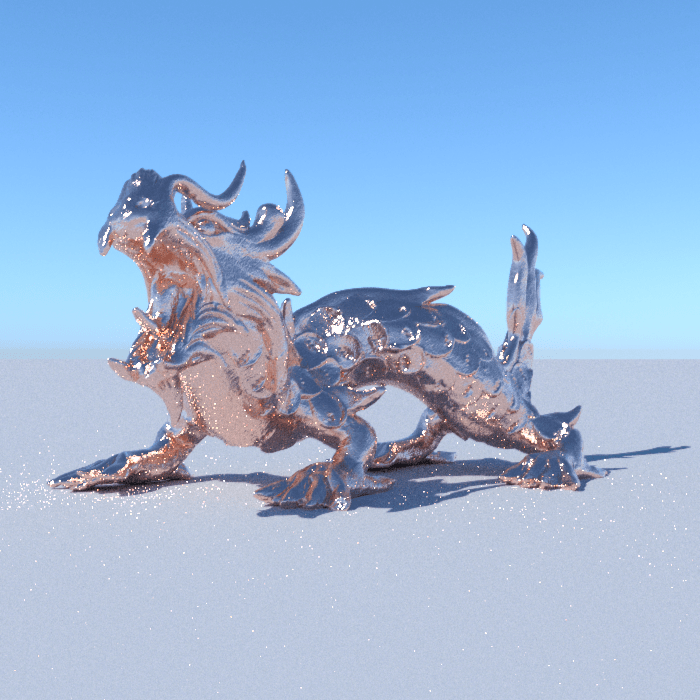
\includegraphics[width=.3\textwidth]{img/4 results/ply/dragonEmbree.png}\label{fig:mesh_dragon}}
	\hfill
	\subfloat[Lucy - 28,055,742 faces ]{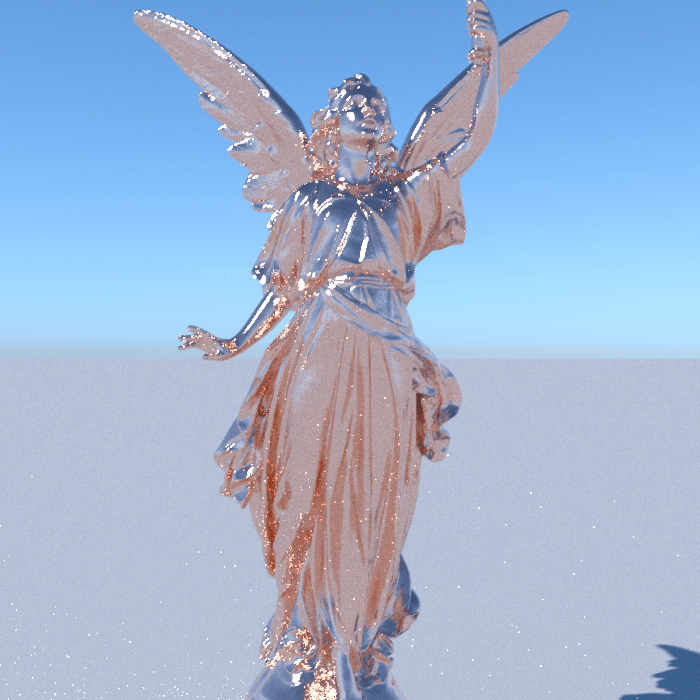
\includegraphics[width=.3\textwidth]{img/4 results/ply/lucyEmbree.png}\label{fig:mesh_lucy}}
	
	\caption{Scenes for triangle meshes}
	\label{fig:mesh_scenes}
\end{figure}

\begin{table}
	\centering
	{\footnotesize\sf
		\begin{tabular}{lrrrr}
			\toprule
			Scene & \Verb!#!Triangles & Native ART & Embree & Speedup \\ 
			\midrule
			Figure \ref{fig:mesh_teapot} & 4,032 & 728.12 sec & 608.29 sec & 16.46 \% \\
			Figure \ref{fig:mesh_bunny} & 69,451 & 379.02 sec & 305.00 sec & 19.53 \% \\
			Figure \ref{fig:mesh_mike} & 366,011 & 302.52 sec & 254.03 sec & 16.03 \%  \\
			\addlinespace % a nice non-intrusive separator of data groups (or final table sums)
			Figure \ref{fig:mesh_buddha} & 1,087,716 & 351.92 sec & 276.00 sec & 21.57 \% \\
			Figure \ref{fig:mesh_dragon} & 7,219,045 & (no data) & 304.29 sec & (no data)  \\
			Figure \ref{fig:mesh_lucy} & 28,055,742 & (no data) & 327.59 sec & (no data)  \\
			\bottomrule
	\end{tabular}}
	\caption{An example table. Table caption should clearly explain how to interpret the data in the table. Use some visual guide, such as boldface or color coding, to highlight the most important results (e.g., comparison winners).}
	\label{tab:mesh}
\end{table}






Rendering triangles and quads, meh.

Not working with Triangle meshes.

